\section{General Circuit}


As explain before two or more operation can be bound to the same resource. Before we bond them together we need to ensure that they are \textit{compatible}. Two conditions that the operations should met in order to be \textit{compatible} :

\begin{itemize}
\item The operations is not concurrent.
\item The operations can be implemented by resources of the same type.
\end{itemize}

So, $ E+\{(v_{i},v_{j})|\tau(v_{i}=v_{j} $ and $ ((t_{i}=d_{i} \leq t_{j}) $ or $ t_{j}=d{j} \leq t_{i})),i,j=1,...,n_{ops}\}$ %


\subsection{Register Sharing}

Register is used by a circuit to store values of variable. Since variable have life time it can be interval. This varable value will be use letter by other operation as an input
\ref{fig:Sequencing_graph_fragment}
\begin{figure}[h]
    \centering
    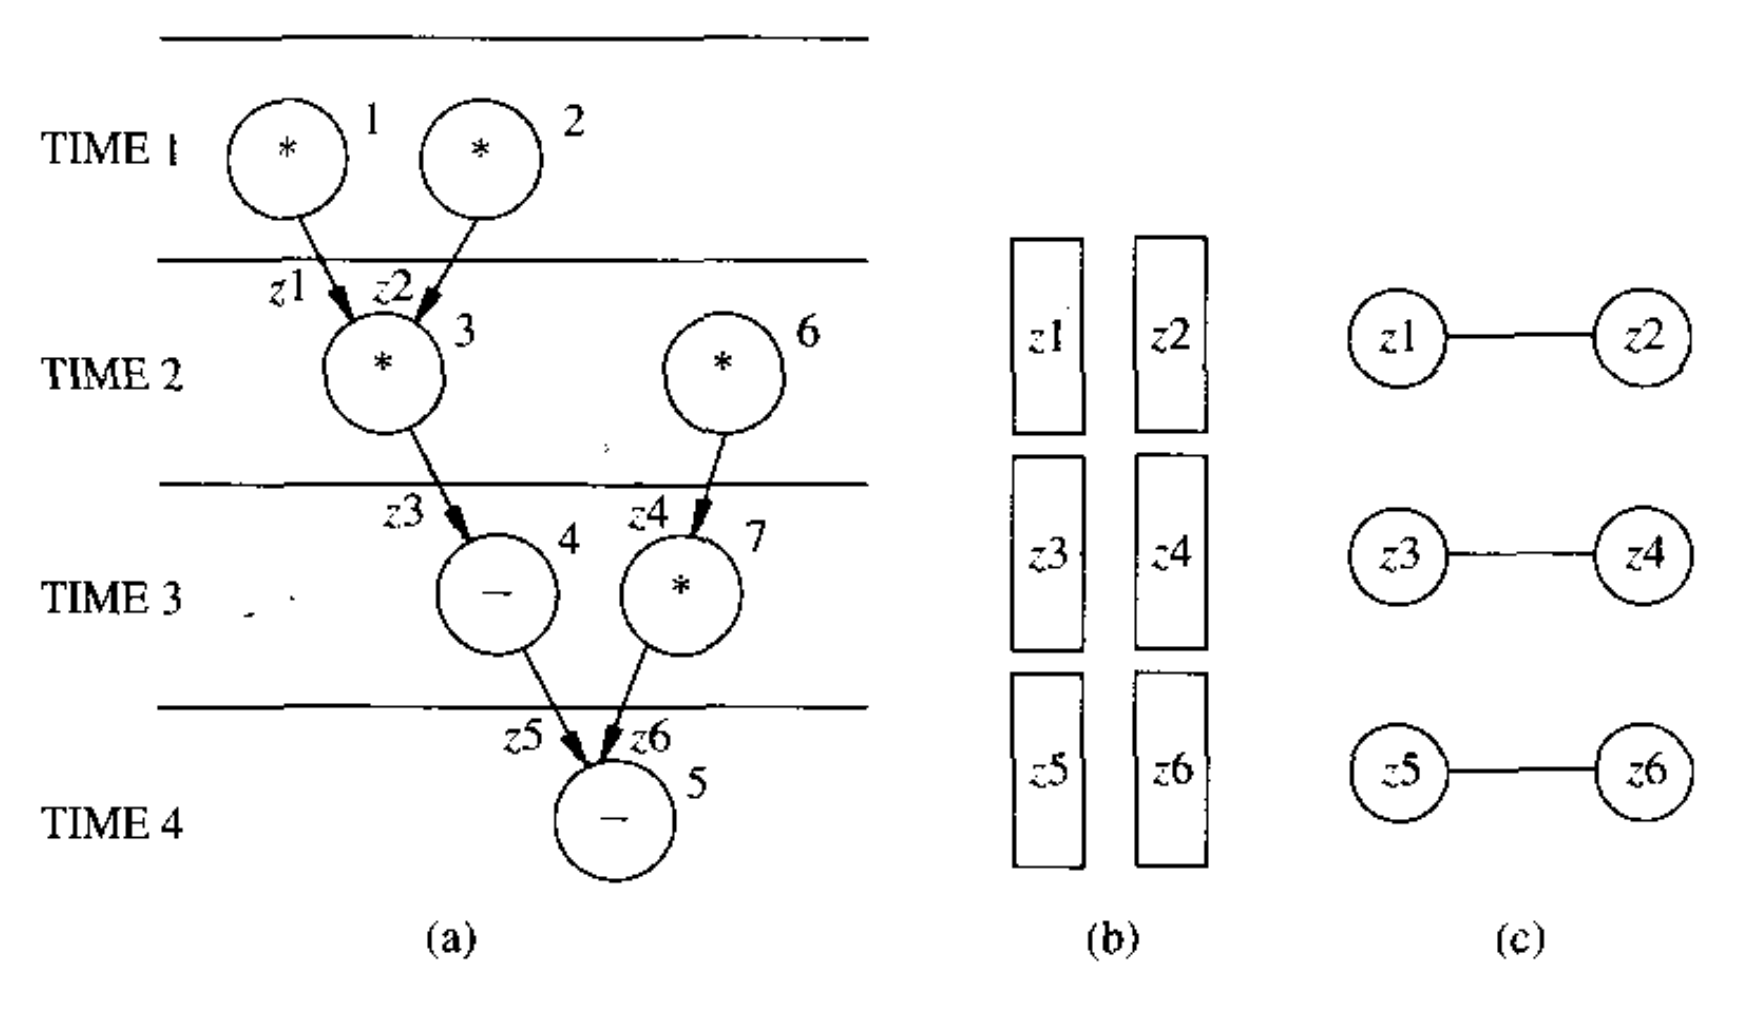
\includegraphics[width=0.5\textwidth]{Sequencing_graph_fragment}
    \caption{ a) Sequencing graph fragment. (b) Variable intervals. (c) Conflict mph \cite{b1}}
    \label{fig:Sequencing_graph_fragment}
\end{figure}

\ref{fig:Sequencing_graph}
\begin{figure}[h]
    \centering
    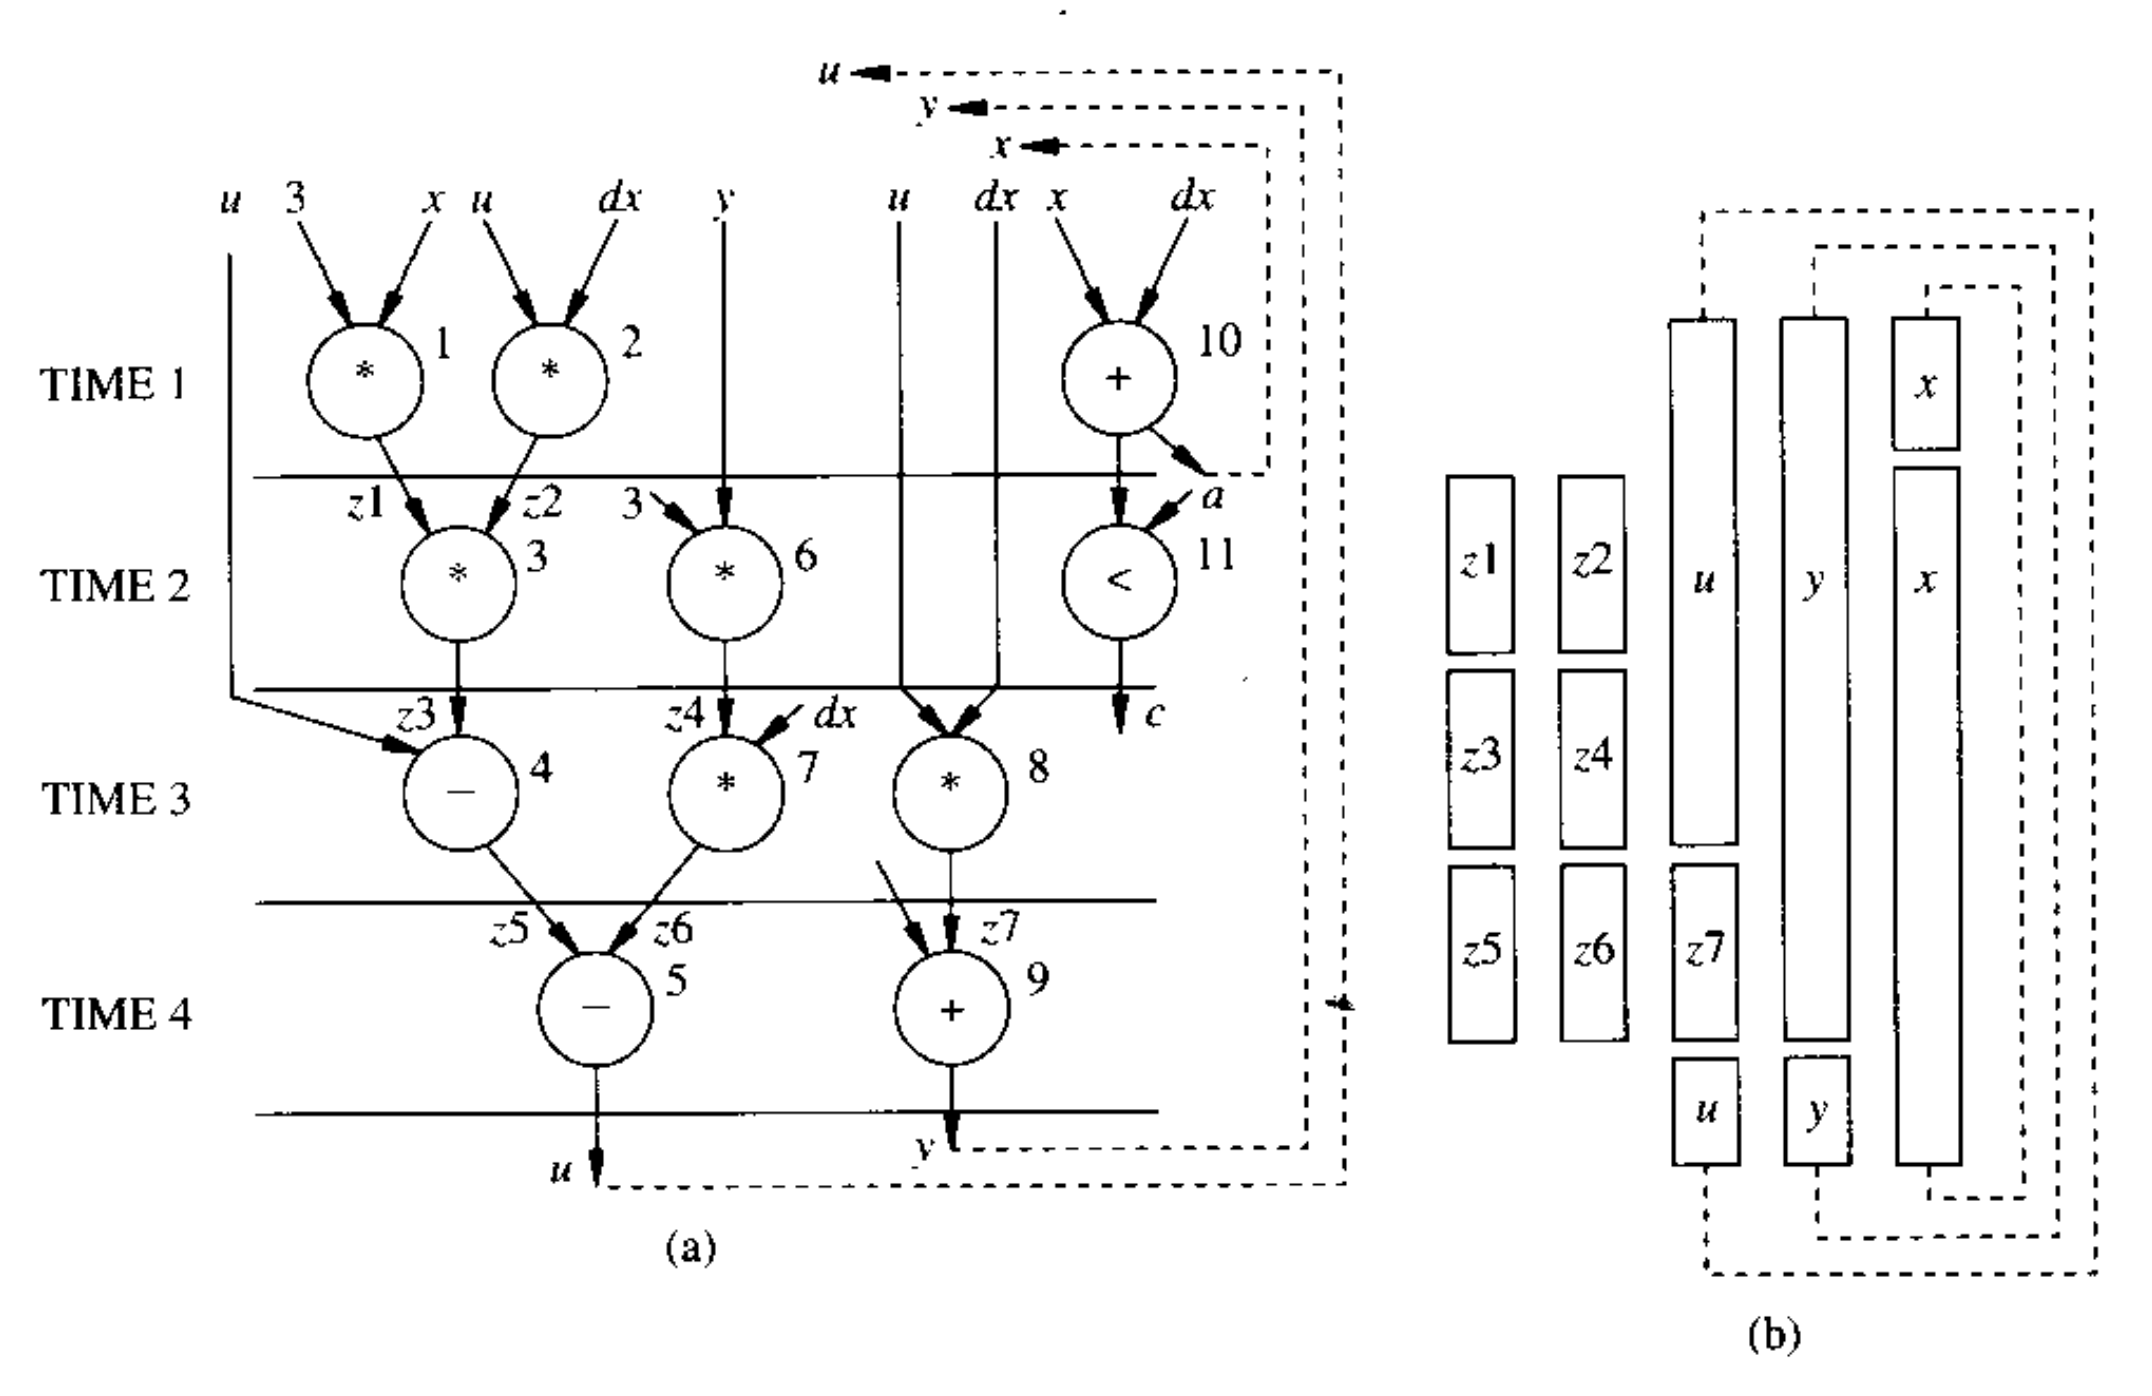
\includegraphics[width=0.5\textwidth]{Sequencing_graph}
    \caption{ (a) Sequencing graph. (b) Variable lifetimes \cite{b1}}
    \label{fig:Sequencing_graph}
\end{figure}

\ref{fig:Variable_lifetimes_as_arcs_on_a_circle}
\begin{figure}[h]
    \centering
    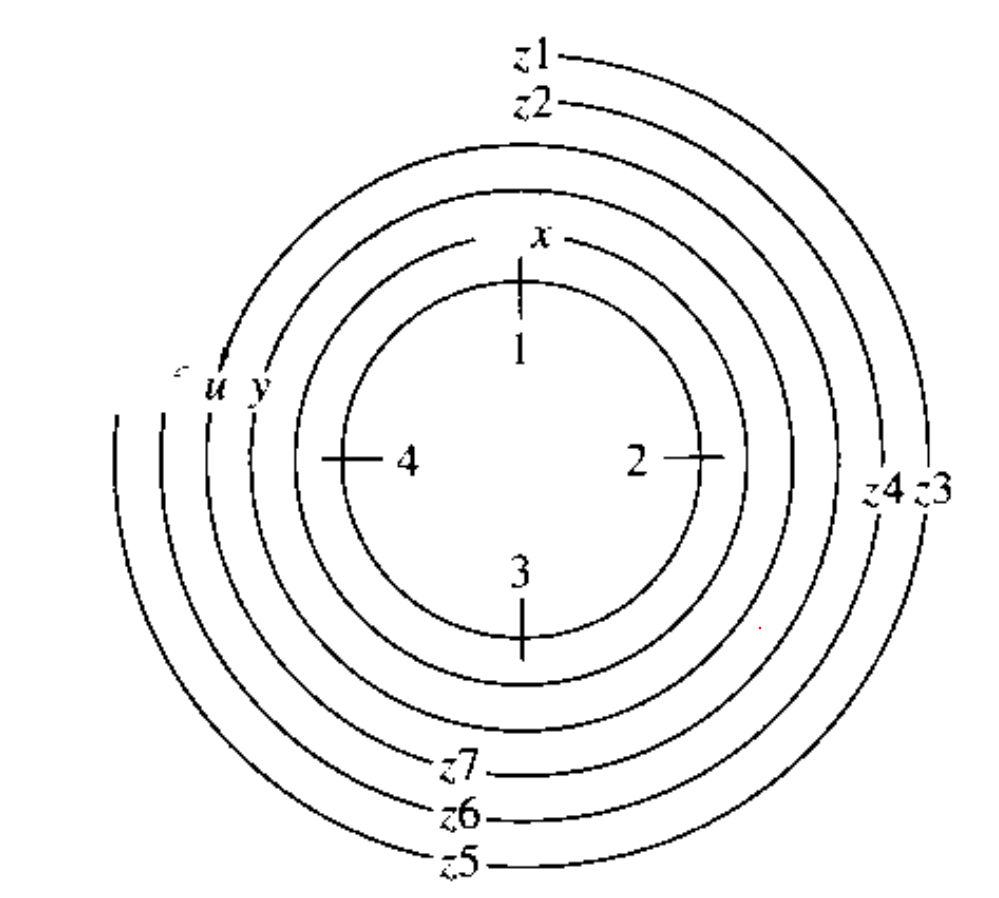
\includegraphics[width=0.4\textwidth]{Variable_lifetimes_as_arcs_on_a_circle}
    \caption{ Variable lifetimes as arcs on a circle \cite{b1}}
    \label{fig:Variable_lifetimes_as_arcs_on_a_circle}
\end{figure}

\ref{fig:Circular_arc_confliCr_graph}
\begin{figure}[h]
    \centering
    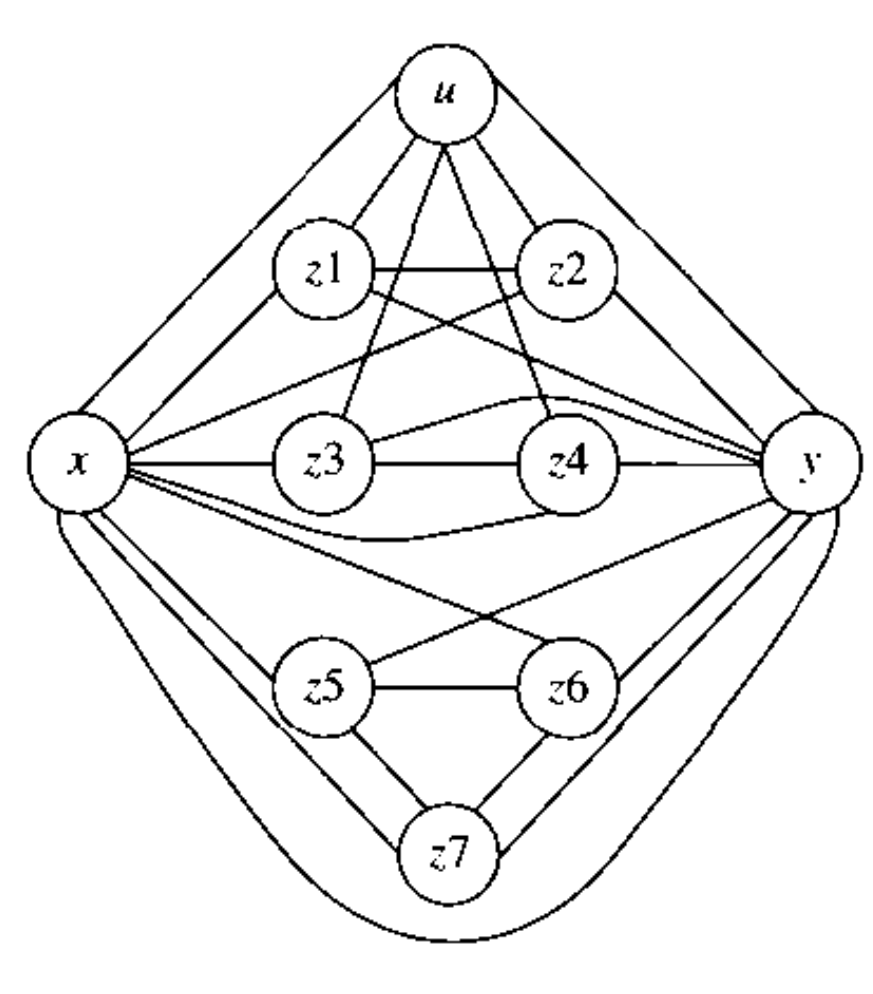
\includegraphics[width=0.4\textwidth]{Circular_arc_confliCr_graph}
    \caption{ Circular-arc conflict graph \cite{b1}}
    \label{fig:Circular_arc_confliCr_graph}
\end{figure}

\subsection{Multiple Memory Binding}

number of port $\geq \underset{1\leq l \leq \lambda + 1}{\mathrm{max} \sum_{i=1}^{n_{var}} x_{il}} $
$ \mathds{1}^{T} b = \sum_{i=l}^{n_{var}}b_{i}$
$ \sum_{i=l}^{n_{var}}b_{i}x_{il}\leq a,l=1,2,..,\lambda+1 $
$ b^{T}=[b_{1},b_{2},...,b_{n_{var}}],b_{i}=1 $
\subsection{Bus Sharing Binding}

\subsection{Multiplexer}
$ n $
$ a $
$ area_{mux} $
$ area_{mux}^{\bigtriangleup} $
$area_{mux} \approx area_{mux}^{\bigtriangleup}(i-1) $

$ area(area_{add}+area_{mux})\approx a(area_{add}- area_{mux}^{\bigtriangleup})+n \cdot area_{mux}^{\bigtriangleup}  $

$ area\approx a\cdot (area_{add}+(\frac{n}{a}-1)) \cdot area_{mux}^{\bigtriangleup} $

$ area_{add} > area_{mux}^{\bigtriangleup} $


$area_{mux} = (i-1)\cdot area_{mux}^{\bigtriangleup} $
$=-area_{mux}^{\bigtriangleup} + i \cdot area_{mux}^{\bigtriangleup}  $
$=area_{M}^{0} + sum_{j=1}{i} area_{M}^{j}$
$ area_{M}^{0} = -areaarea_{mux}^{\bigtriangleup} $
$ area_{M}^{j}=area_{mux}^{\bigtriangleup} $


\ref{fig:Comparibility_graph_mux}
\begin{figure}[h]
    \centering
    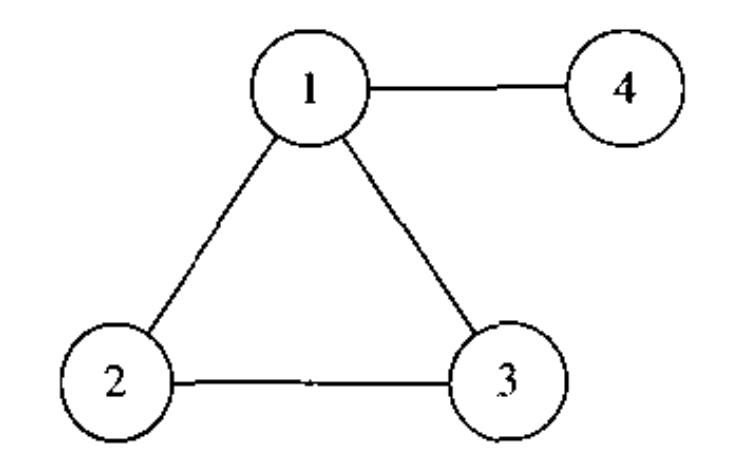
\includegraphics[width=0.3\textwidth]{Comparibility_graph_mux}
    \caption{ Compatibility graph \cite{b1}}
    \label{fig:Comparibility_graph_mux}
\end{figure}

\ref{fig:Comparibility_graph_mux_2}
\begin{figure}[h]
    \centering
    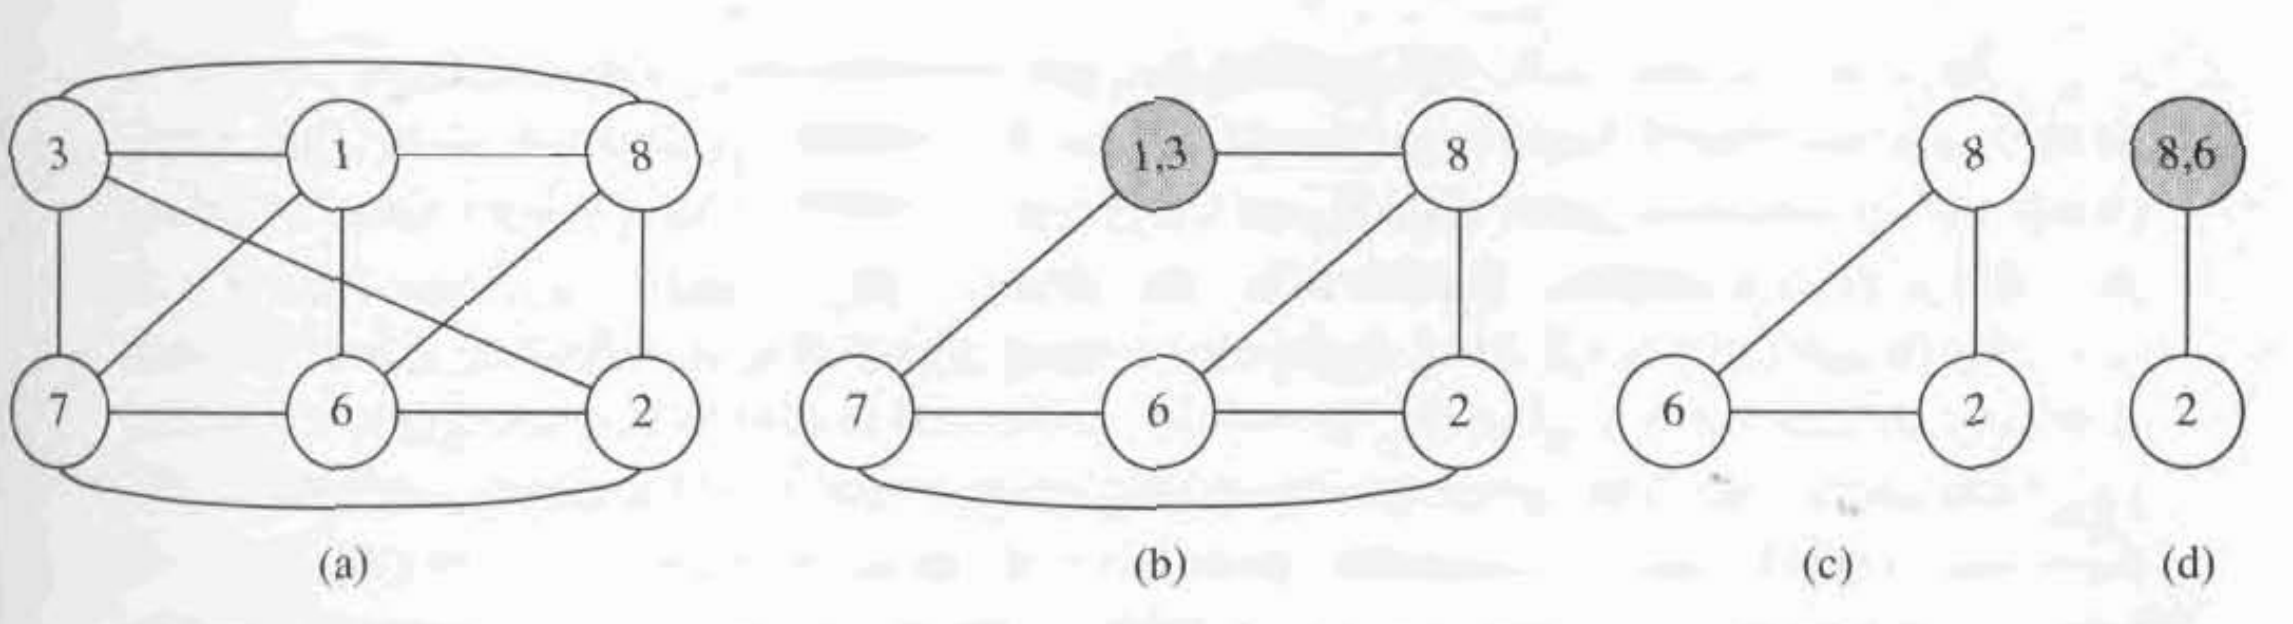
\includegraphics[width=0.5\textwidth]{Comparibility_graph_mux_2}
    \caption{ (a) Compatibility graph for the multiplier type. (b) Reduced compatibility graph with clique seed. (c) Fragment of compatibility graph after one clique has heen removed. (d) Reduced fragment with clique seed. \cite{b1}}
    \label{fig:Comparibility_graph_mux_2}
\end{figure}

\subsection{Performance-Constraint}

$ path_delay=sum_{i \in path}^{}d_{i} + mux_delay(B)+wire_delay(B)< \phi $
$ c^{T}a $
$ d_{i} $
$ B $
$ \phi $

\subsection{Performance-Directed Binding}

%	register sharing
%		lifetime variable
%		variable alive in non overlaping intervals or under alternative condition are compatible
%		compatibility graph
%		conflict graph
%		non-hierarchical
%		hierarchical
%	multiple memory binding
%	
%	bus sharing and bnding
%	
%	multiplexer